
\chapter{TINJAUAN PUSTAKA}


\section{Landasan Teori}

\subsection{Citra Digital}
Citra digital dapat didefinisikan sebagai fungsi \textit{f(x,y)} berukuran M baris dan N kolom, dengan \textit{x} dan \textit{y} adalah koordinat spasial, dan amplitudo \textit{f} di titik koordinat (x,y) dinamakan intensitas atau tingkat keabuan dari citra pada citra tersebut \cite{book:darma}. Pada umumnya warna dasar dalam citra RGB menggunakan penyimpanan 8 bit untuk menyimpan data warna, yang berarti setiap warna mempunyai gradasi sebanyak 255 warna . Dewasa ini, citra digital dapat menggunakan 16 bit untuk menyimpan data warna dasarnya, hal ini menyebabkan semakin banyak gradasi warnanya sehingga citra yang dihasilkan memiliki tingkat warna yang jauh lebih banyak. Namun tentu saja hal ini mengakibatkan ukuran file citra digital yang dihasilkan juga menjadi semakin besar walaupun dengan ukuran yang sama. Berdasarkan jenis warnanya citra digital dibagi menjadi 3 jenis yaitu citra biner, citra grayscale dan citra warna.

\subsubsection{Citra Biner (monokrom)} 
Citra biner adalah citra yang hanya memiliki dua warna saja yaitu hitam dan putih. Warna hitam direpresentasikan dengan 1 dan warna putih direpresentasikan dengan 0. Dibutuhkan 1 bit di memori untuk menyimpan nilai warna pada setiap piksel citra biner. Contoh citra biner dapat dilihat pada gambar ~\ref{fig:jenis-citra}(a).

\subsubsection{Citra Grayscale}
Banyaknya warna pada citra \textit{grayscale} tergantung pada jumlah bit yang disediakan di memori untuk menampung kebutuhan warna pada citra ini. Citra \textit{grayscale} yang 2 bit memiliki 4 gradasi warna, citra \textit{grayscale} 3 bit memiliki 8 gradasi warna, citra \textit{grayscale} dengan 8 bit memiliki 256 gradasi warna dan seterusnya. Semakin besar jumlah bit warna yang disediakan di memori, semakin banyak dan semakin halus gradasi warna yang terbentuk. Pada umumnya citra digital \textit{grayscale} menggunakan 8 bit memori dengan derajat keabuan dari 0 sampai 255. Contoh citra \textit{grayscale} dapat dilihat pada gambar ~\ref{fig:jenis-citra}(b).

\subsubsection{Citra Warna} 
Setiap piksel pada citra warna mewakili warna yang merupakan kombinasi dari tiga warna dasar (RGB = red, green, blue). Pada umumnya setiap warna dasar menggunakan penyimpanan 8 bit, yang berarti setiap warna mempunyai gradasi sebanyak 255 warna. Berarti setiap piksel mempunyai kombinasi warna sebanyak 255 x 255 x 255 =16 juta warna lebih. Contoh citra warna dapat dilihat pada gambar ~\ref{fig:jenis-citra}(c).

\begin{afigure}
    \includegraphics[width=0.85\textwidth, center]{images/jenis-jenis-citra.png}
    \caption{(a) Contoh citra biner, (b) contoh citra grayscale, (c) contoh citra warna.}
    \label{fig:jenis-citra}
\end{afigure}


\subsection{Pengolahan Citra Digital}
Pengolahan citra digital merupakan proses mengolah piksel-piksel di dalam citra secara digital untuk tujuan tertentu. Berdasarkan tingkat pemrosesannya pengolahan citra digital dikelompokkan menjadi tiga kategori, yaitu: \textit{low-level}, \textit{mid-level} dan pemrosesan \textit{high-level}. Pemrosesan \textit{low-level} dilakukan dengan operasi primitif seperti \textit{image preprocessing} untuk mengurangi derau (\textit{noise}), memperbaiki kontras citra dan mempertajam citra (\textit{sharpening}). Karakteristik dari pemrosesan \textit{low-level} yaitu keluaran atau hasil dari pemrosesannya berupa citra digital. Pemrosesan \textit{mid-level} melibatkan tugas-tugas seperti segmentasi (mempartisi gambar menjadi beberapa bagian atau objek), deskripsi objek untuk dilakukan pemrosesan lanjutan, dan klasifikasi objek dalam citra digital. Karakteristik dari pemrosesan \textit{mid-level} yaitu keluaran atau hasilnya berupa atribut atau fitur seperti, kontur, tepi, atau objek yang terdapat dalam citra tersebut. Pemrosesan \textit{high-level} merupakan proses tingkat lanjut dari dua proses sebelumnya, dilakukan untuk mendapat informasi lebih yang terkandung dalam citra \cite{book:gonzalez}.

Berdasarkan tujuannya pengolahan citra juga dapat dibagi menjadi beberapa bagian yaitu: \textit{image enhancement}, \textit{image restoration}, \textit{image analysis} dan \textit{image compression} \cite{book:dasilva}.

\subsubsection{Image Enhancement}
\textit{Image Enhancement} adalah metode pengolahan citra digital untuk membuat citra tampak lebih baik atau dilakukan peningkatan untuk analisis tertentu. Namun hal ini dapat menyebabkan pengorbanan aspek lain dari citra tersebut. Penerapan filter, penghalusan citra, memperbaiki kontras dan morfologi citra adalah contoh \textit{image enhancement}.

\subsubsection{Image Restoration}
\textit{Image restoration} adalah metode pengolahan citra untuk memulihkan citra dari penurunan kualitas atau citra yang rusak karena derau (\textit{noise}). Pada dasarnya metode ini berbeda dengan \textit{image enhancement} yang berkaitan dengan ekstraksi fitur pada citra. 

\subsubsection{Image Analysis}
\textit{Image analysis} adalah metode pengolahan citra untuk menghitung besaran kuantitatif dari citra untuk menghasilkan deskripsinya. Metode ini dilakukan dengan mengekstraksi ciri-ciri tertentu yang membantu dalam identifikasi objek \cite{book:dasilva}.

\subsubsection{Image Compression}
Metode ini dilakukan agar citra dapat direpresentasikan dalam bentuk yang lebih kompak sehingga memerlukan memori yang lebih sedikit. Metode ini dapat dilakukan dengan mengurangi redundansi dari data-data yang terdapat dalam citra sehingga dapat disimpan atau ditransmisikan secara efisien.


\subsection{Filter Spasial}
Konsep filter spasial pada pengolahan citra digital berasal dari penerapan transformasi Fourier untuk pemrosesan sinyal pada domain frekuensi. Istilah filter spasial ini digunakan untuk membedakan proses ini dengan filter pada domain frekuensi. Proses filter dilakukan dengan cara menggeser filter kernel dari titik ke titik dalam citra digital. Istilah \textit{mask}, \textit{kernel}, \textit{template}, dan \textit{window} merupakan istilah yang sama dan sering digunakan dalam pengolahan citra digital \cite{book:gonzalez}. Dalam penelitian ini peneliti menggunakan istilah kernel untuk istilah tersebut.

Proses filter dalam pengolahan citra digital dilakukan dengan memanipulasi sebuah citra menggunakan kernel untuk menghasilkan citra yang baru, sehingga dengan kernel yang berbeda maka citra hasil yang didapat juga akan berbeda. 


\subsubsection{Operator Linear dan Non-linear}
Didefinisikan H sebuah operator dengan \textit{input} dan \textit{output} adalah citra digital. H dikatakan operator linear jika untuk untuk sembarang gambar \textit{f} dan \textit{g}, dan untuk sembarang skalar a dan b berkalu,
\begin{equation}
    \label{eq:linearity-operator}
    H(af + bg) = aH(f) + bH(g)
\end{equation}

Dengan kata lain hasil dari operator linear dengan jumlahan dua buah citra (yang telah dikali dengan konstanta a dan b) identik dengan hasil operator linear pada masing-masing gambar, dikali dengan konstanta yang sama, kemudian hasilnya dijumlahkan. Sebagai contoh, sebuah operator dengan fungsi yang menjumlahkan K citra adalah operator linear. Operator yang menghitung nilai mutlak dari perbedaan dua gambar adalah tidak linear. Operator yang tidak memenuhi persamaan (\ref{eq:linearity-operator}) dikatakan non-linear \cite{book:gonzalez}.


\subsection{Kernel}

\subsubsection{Average Blur}
\textit{Average blur} atau biasa juga disebut \textit{box filter} adalah salah satu filter yang digunakan untuk menghaluskan citra dan mengurangi derau. Secara sederhana nilai sebuah piksel yang baru adalah nilai rata-rata dari nilai piksel tersebut dengan nilai piksel tetangganya \cite{pdf:marcin}. Berikut kernel \textit{Average blur} yang digunakan dalam penelitian ini:
\begin{equation}
    \label{kernel:average}
    \frac{1}{9} \left[
    \begin{matrix}
 1 & 1 & 1 \\
 1 & 1 & 1 \\
 1 & 1 & 1
    \end{matrix}
    \right]
\end{equation}

\subsubsection{Gaussian Blur}
Filter ini juga digunakan untuk menghaluskan citra dan mengurangi derau. Idenya mirip seperti \textit{Average blur}, nilai piksel yang baru dibentuk dari nilai piksel tetangganya, tetapi dengan memberikan bobot yang lebih kuat pada nilai pikselnya sendiri diikuti dengan bobot yang lebih rendah pada piksel atas, bawah dan sampingnya \cite{soa:dmitry}. Berikut kernel gaussian blur filter yang digunakan dalam penelitian ini:
\begin{equation}
    \label{kernel:gaussianblur}
    \frac{1}{16}
    \left[
    \begin{matrix}
 1 & 2 & 1 \\
 2 & 4 & 2 \\
 1 & 2 & 1
    \end{matrix}
    \right]
\end{equation}

\subsubsection{Sobel}
Filter Sobel termasuk \textit{high-pass} filter yang umum digunakan untuk deteksi tepi pada citra. Sobel memiliki dua kernel untuk deteksi tepi yaitu kernel sobel vertikal untuk mendeteksi tepi secara vertikal dan kernel sobel horizontal yang mendeteksi tepi secara horizontal \cite{pdf:marcin}. Berikut kernel Sobel vertikal dan horizontal yang digunakan dalam penelitian ini:
\begin{equation}
    \label{kernel:sobel}
    \left[
    \begin{matrix}
 1 & 0 & -1 \\
 2 & 0 & -2 \\
 1 & 0 & -1
    \end{matrix}
    \right]
    \hspace{2cm}
    \left[
 \begin{matrix}
 1 & 2 & 1 \\
 0 & 0 & 0 \\
 -1 & -2 & -1
    \end{matrix}
    \right]
\end{equation}

\subsubsection{Laplacian}
Filter ini dapat digunakan untuk deteksi tepi pada citra karena sifatnya yang sensitif dengan perubahan intensitas yang cepat \cite{pdf:jingbo}. Tidak seperti Sobel yang menggunakan dua kernel untuk mendeteksi tepi secara vertikal dan horizontal, disini hanya digunakan sebuah kernel yang dapat digunakan untuk deteksi tepi secara vertikal dan horizontal sekaligus. Berikut kernel Laplacian yang digunakan dalam penelitian ini:
\begin{equation}
    \label{kernel:laplacian}
    \left[
    \begin{matrix}
 0 & 1 & 0 \\
 1 & -4 & 1 \\
 0 & 1 & 0
    \end{matrix}
    \right]
\end{equation}

\subsubsection{Sharpening}
Sharpening filter digunakan untuk memperjelas detail halus dalam citra atau untuk meningkatkan detail pada citra yang \textit{blur}, baik karena kesalahan ataupun karena efek dari metode akuisisi citra tertentu \cite{pdf:ching}. Berikut kernel untuk filter \textit{sharpening} yang digunakan dalam penelitian ini:
\begin{equation}
    \label{kernel:sharpen}
    \left[
    \begin{matrix}
 -1 & -1 & -1 \\
 -1 & 9 & -1 \\
 -1 & -1 & -1
    \end{matrix}
    \right]
\end{equation}


\subsection{Konvolusi}
Konsep filter spasial linear mirip seperti konsep konvolusi pada domain frekuensi, dengan alasan tersebut filter spasial linear biasa disebut juga konvolusi sebuah kernel dengan citra digital \cite{book:gonzalez}. Konvolusi pada fungsi \textit{f(x)} dan \textit{g(x)} didefinisikan pada persamaan \ref{eq:conv1}.
\begin{equation}
    \label{eq:conv1}
    \begin{split}
h(x) = f(x) * g(x) = \int_{-\infty}^{\infty} f(a) g(x-a) da
    \end{split}
\end{equation}
dimana tanda * menyatakan operator konvolusi, dan peubah a adalah peubah bantu. Untuk fungsi diskrit, konvolusi didefinisikan pada persamaan \ref{eq:conv2}.
\begin{equation}
    \label{eq:conv2}
    \begin{split}
h(x) = f(x) * g(x) = \sum_{a=-\infty}^{\infty} f(a)g(x-a)
    \end{split}
\end{equation}

Pada operasi konvolusi diatas, \textit{g(x)} disebut kernel konvolusi atau filter kernel. Kernel \textit{g(x)} dioperasikan secara bergeser pada sinyal masukan \textit{f(x)}. Jumlah perkalian kedua fungsi pada setiap titik merupakan hasil konvolusi yang dinyatakan dengan keluaran \textit{h(x)} \cite{book:munir}. 

Pada gambar (\ref{fig:conv3}) diilustrasikan bagaimana proses konvolusi pada citra digital yang direpresentasikan dalam bentuk matriks. Operasi konvolusi dilakukan pada matriks input berukuran 6x6 dengan filter berukuran 3x3. Hasil konvolusinya ditampilkan pada matriks \textit{result}.
\begin{afigure}
    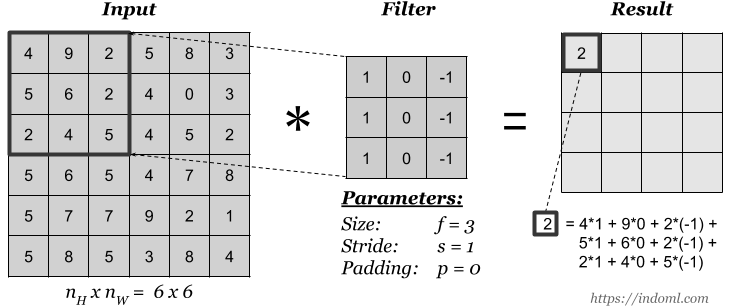
\includegraphics[width=0.85\textwidth, center]{images/convolution-operation.png}
    \caption{Ilustrasi konvolusi pada citra. Sumber: https://indoml.com}
    \label{fig:conv3}
\end{afigure}

Jika hasil konvolusi menghasilkan nilai piksel negatif, maka nilai tersebut dijadikan 0, sebaliknya jika hasil konvolusi menghasilkan nilai piksel yang melebihi nilai keabuan maksimum, maka nilai tersebut dijadikan ke nilai keabuan maksimum pada citra tersebut \cite{book:sutoyo}.
% masalah padding
 

\subsection{Video Stream}
Video \textit{stream} dapat dipandang sebagai serangkaian citra digital berturut-turut \cite{thesis:jin}. Berbeda dengan format video lainya, video \textit{stream} ini tidak disimpan pada media penyimpanan sebagai file dengan format video melainkan langsung disalurkan setiap framenya dari sumber (\textit{source}) ke penerima, dalam hal ini FPGA.  Dengan menganggap Video \textit{stream} adalah kumpulan citra digital (\textit{frame}) maka dapat dilakukan metode pengolahan seperti pada citra digital, termasuk penerapan filter spasial. 


\subsection{FPGA}
\textit{Field Programmable Gate Arrays} atau FPGA adalah perangkat semikonduktor yang berbasis \textit{matriks configurable logic block} (CLBs) yang terhubung melalui interkoneksi yang dapat diprogram. FPGA dapat diprogram ulang ke aplikasi atau fungsi yang diinginkan setelah \textit{manufacturing}. Fitur ini yang membedakan FPGA dengan \textit{Application Specific Integrated Circuits} (ASICs), yang dibuat khusus untuk tugas tertentu saja \cite{XILINX}.

Sebuah \textit{microprocessor} menerima instruksi berupa kode 1 atau 0, kode-kode ini selanjutnya diinterpretasikan oleh komputer untuk menjalankan perintah yang diberikan. \textit{Microprocessor} ini membutuhkan intruksi berupa kode secara terus menerus untuk menjalankan fungsinya. Sedangkan pada FPGA hanya dibutuhkan sekali konfigurasi \textit{chip} setiap kali dinyalakan. Membuat atau mengunduh \textit{bitstream} yang menentukan fungsi logika dilakukan oleh \textit{logic elements} (LEs), sebuah sirkuit dapat dibuat dengan menggabungkan beberapa LEs menjadi satu kesatuan. Setelah \textit{bitstream} dipasang, FPGA tidak perlu lagi membaca instruksi berupa 1 dan 0, berbeda dengan \textit{microprocessor} yang selalu membutuhkan instruksi \cite{pdf:cheung}. Secara tradisional, untuk membuat sebuah desain FPGA, aplikasi dideskripsikan menggunakan \textit{Hardware Description Language} (HDL) seperti Verilog atau VHDL sehingga menghasilkan sebuah \textit{bitstream} FPGA. 

\begin{afigure}
    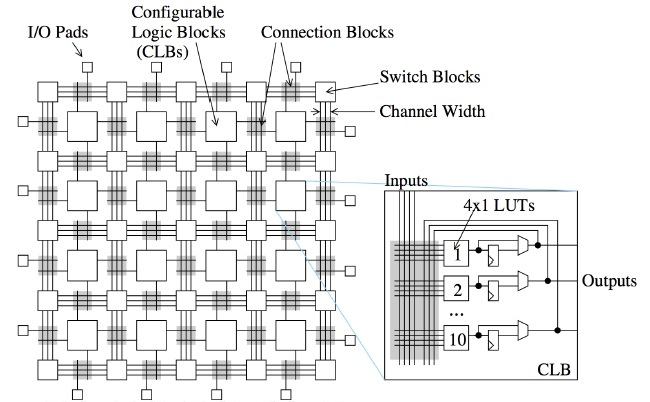
\includegraphics[width=12cm, center]{images/fpga-structure.jpeg}
    \caption{Struktur FPGA.}
    \label{fig:fpga-structure}
\end{afigure}

\subsubsection{FPGA Development Board}
Pada FPGA terdahulu tidak terdapat \textit{processor} (CPU) untuk menjalankan software apapun, sehingga ketika ingin mengimplementasikan aplikasi haruslah merancang sirkuit dari awal, seperti mengonfigurasi FPGA sesederhana gerbang logika OR atau serumit \textit{multi-core processor} \cite{site:biswas}. Dewasa ini telah dikembangkan FPGA \textit{Development Board} atau biasa disebut juga FPGA \textit{Board} yaitu teknologi FPGA yang dirangkai dalam sebuah \textit{board} dan dilengkapi dengan \textit{microprocessor} dan beberapa \textit{interface} \textit{IO} untuk menjalankan tugas tertenu. Umumnya FPGA \textit{Board} telah dilengkapi dengan interface untuk mengakses dan menerapkan desain sirkuitnya. Xilinx, Altera dan Intel adalah produsen FPGA \textit{Board} yang terkenal. FPGA \textit{Board} yang digunakan dalam penelitian ini yaitu Xilinx PYNQ-Z2 dengan Jupyter Notebook sebagai \textit{interface} untuk mengakses dan menjalankan program pada penelitian ini. Bentuk FPGA \textit{Board} Xilinx PYNQ-Z2 dapat dilihat pada gambar (\ref{fig:pynq-z2})

\begin{afigure}
    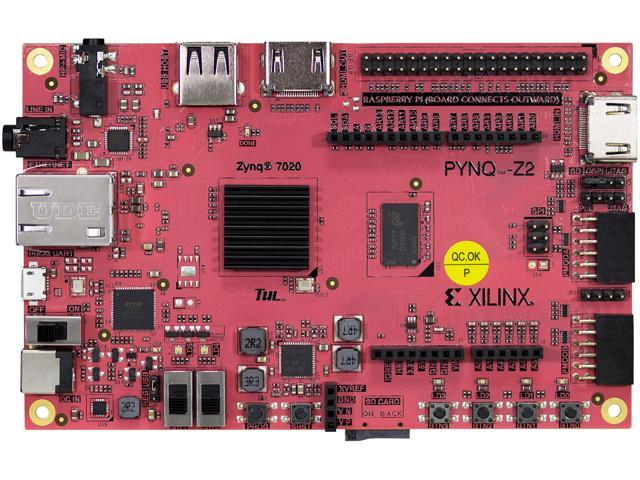
\includegraphics[width=10cm, center]{images/pynq-z2.jpeg}
    \caption{FPGA Board Xilinx PYNQ-Z2.}
    \label{fig:pynq-z2}
\end{afigure}


\subsection{Evaluasi Kinerja}
Pada penelitian ini peneliti menggunakan waktu komputasi, \textit{frame rate} (FPS), penggunaan CPU, penggunaan {memory}, penggunaan {resident memory} (RES), {shared memory} (SHR), dan {virtual memory} (VIRT) untuk mengukur kinerja pada penerapan filter spasial linear dengan prosesor ARM dan FPGA.

\subsubsection{Waktu Komputasi}
Waktu komputasi yang dimaksud oleh peneliti adalah durasi yang dibutuhkan sebuah kernel untuk melakukan filter spasial linear terhadap beberapa \textit{frame} input. Waktu komputasi ini diperoleh dengan cara menghitung selisih waktu selesai dengan waktu dimulai penerapan filter spasial linear pada \textit{frame} input.
% \cite{pdf:chang}
\begin{equation}
    \label{eq:time}
    \begin{split}
waktu\ kompuatsi = waktu\ selesai - waktu\ mulai
    \end{split}
\end{equation}

\subsubsection{Frame Rate (FPS)}
\textit{Frame rate} atau \textit{frame per second} (fps) adalah banyaknya \textit{frame} yang ditampilkan per detik pada video ataupun video \textit{straem}. Semakin tinggi fps sebuah video maka semakin halus pula gerakan yang dihasilkan. Sebaliknya video dengan fps rendah akan menghasilkan gerakan yang kurang baik. \textit{Frame rate} atau fps dapat dihitung dengan cara membagi jumlah \textit{frame} dengan waktu komputasinya seperti pada persamaan \ref{eq:fps} \cite{pdf:pavan}.
\begin{equation}
    \label{eq:fps}
    \begin{split}
fps = \frac{jumlah\ frame}{waktu\ komputasi}
    \end{split}
\end{equation}

\subsubsection{Penggunaan CPU}
Pada penelitian ini peneliti menggunakan fitur yang tersedia pada sistem operasi Linux yang berjalan di FPGA Development Board untuk melihat persentase penggunaan CPU pada proses penerapan filter spasial linear. Tampilan dari program ini dapat dilihat pada gambar \ref{fig:top}. Program ini menampilkan informasi tentang proses-proses yang berjalan pada sistem operasi seperti ID sebuah proses, user yang menjalankan proses tersebut, \textit{memory} yang digunakan, status sebuah proses, persentase CPU yang digunakan dan lainnya.
\begin{figure}[H]
    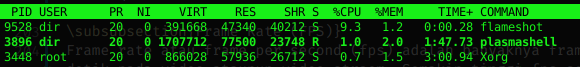
\includegraphics[width=0.9\textwidth, center]{images/programs/top.png}
    \caption{Tampilan program top pada Linux.}
    \label{fig:top}
\end{figure}
Status sebuah proses pada program ini dinyatakan dengan beberapa singkatan, diantaranya yaitu:
\begin{itemize}[noitemsep, topsep=0pt]
    \item[]{\makebox[0.5cm]{I\hfill} = \textit{idle}}
    \item[]{\makebox[0.5cm]{R\hfill} = \textit{running}}
    \item[]{\makebox[0.5cm]{S\hfill} = \textit{sleeping}}
    \item[]{\makebox[0.5cm]{Z\hfill} = \textit{zombie}}
    \item[]{\makebox[0.5cm]{D\hfill} = \textit{uninterruptible sleep}}
    \item[]{\makebox[0.5cm]{T\hfill} = \textit{stopped by job control signal}}
    \item[]{\makebox[0.5cm]{t\hfill} = \textit{stopped by debugger during trace}}
  \end{itemize}

Pada CPU yang multi-core sebuah proses akan ditampilkan persentase penggunaan CPUnya berdasarkan core yang digunakan oleh proses tersebut. Jika mode Irix pada program \textit{top} dimatikan, maka program akan berjalan pada mode Solaris di mana penggunaan CPU sebuah proses yang ditampilkan akan dibagi dengan jumlah total core yang ada pada CPU \cite{manual:linux}.

\subsubsection{Penggunaan Memory}

Pada sistem operasi linux \textit{memory} dibagi menjadi tiga jenis \cite{manual:linux}. Pertama yaitu \textit{memory} fisik, sumber daya terbatas di mana kode dan data harus berada saat dijalankan atau direferensikan. Berikutnya adalah \textit{memory} \textit{swap}, yaitu  \textit{memory} yang berguna untuk membantu kerja \textit{memory} fisik, data dari \textit{memory} fisik akan disimpan pada \textit{swap} dan kemudian diambil kembali jika terlalu banyak permintaan pada \textit{memory} fisik. Ketiga yaitu virtual \textit{memory}, sumber daya yang hampir tidak terbatas yang digunakan untuk tujuan berikut \cite{book:os}:

\begin{itemize} [noitemsep, topsep=0pt]
    \item \textit{abstraction}, bebas dari alamat / batas \textit{memory} fisik 
    \item \textit{isolation}, setiap proses dalam ruang alamat terpisah 
    \item \textit{sharing}, pemetaan tunggal dapat memenuhi banyak kebutuhan 
    \item \textit{flexibility}, menetapkan alamat virtual ke data 
\end{itemize}

Terlepas dari bentuk \textit{memory} mana yang mungkin digunakan, semua dikelola sebagai \textit{pages} (biasanya 4096
byte). Penggunaan \textit{memory} berhubungan dengan \textit{memory} fisik dan \textit{swap} untuk sistem secara keseluruhan. 
Untuk setiap proses yang berjalan, setiap \textit{memory} page dibatasi ke satu kuadran seperti pada gambar \ref{fig:mem-quad}. Baik \textit{memory} fisik dan \textit{memory} virtual dapat menyertakan salah satu dari empat kuadran, sementara file \textit{swap} hanya mencakup kuadran 1 sampai 3. Memori di kuadran 4, bertindak sebagai file \textit{swap} khusus ketika dimodifikasi \cite{manual:linux}. 

\begin{figure}[H]
    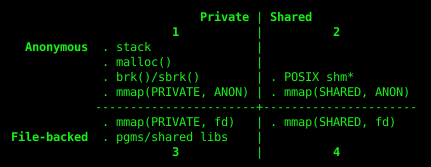
\includegraphics[width=0.8\textwidth, center]{images/programs/memory-quadrant.png}
    \caption{Kuadran pembagian memory pada Linux.}
    \label{fig:mem-quad}
\end{figure}

\subsubsection{Virtual Memory (VIRT)}
Virtual \textit{memory} menggunakan disk sebagai perpanjangan dari RAM sehingga ukuran efektif \textit{memory} yang dapat digunakan bertambah secara bersamaan. Kernel akan menulis konten dari blok \textit{memory} yang saat ini tidak digunakan ke hard disk sehingga \textit{memory} dapat digunakan untuk tujuan lain. Ketika konten asli dibutuhkan lagi, mereka dibaca kembali ke dalam \textit{memory}. Ini semua dibuat transparan sepenuhnya bagi pengguna. Program yang berjalan di Linux hanya melihat jumlah \textit{memory} yang tersedia lebih besar dan tidak memperhatikan bahwa sebagian dari program tersebut berada di disk dari waktu ke waktu. Tentu saja, membaca dan menulis hard disk lebih lambat daripada menggunakan \textit{memory} fisik, sehingga program tidak berjalan secepat itu. Bagian dari hard disk yang digunakan sebagai \textit{memory} virtual disebut ruang swap \cite{site:ltdp}.

% Linux supports virtual \textit{memory}, that is, using a disk as an extension of RAM so that the effective size of usable \textit{memory} grows correspondingly. The kernel will write the contents of a currently unused block of \textit{memory} to the hard disk so that the \textit{memory} can be used for another purpose. When the original contents are needed again, they are read back into \textit{memory}. This is all made completely transparent to the user; programs running under Linux only see the larger amount of \textit{memory} available and don't notice that parts of them reside on the disk from time to time. Of course, reading and writing the hard disk is slower (on the order of a thousand times slower) than using real \textit{memory}, so the programs don't run as fast. The part of the hard disk that is used as virtual \textit{memory} is called the swap space.

Kolom VIRT pada program \textbf{top} menunjukkan jumlah total \textit{memory} virtual yang digunakan oleh proses. Ini mencakup semua kode, data dan \textit{shared  libraries} ditambah dengan \textit{pages} yang telah ditukar dan \textit{pages} yang telah dipetakan tetapi tidak digunakan \cite{manual:linux}. 

% Virtual Memory Size (KiB)
% The total amount of virtual memory used by the task.  It includes all code, data
% and  shared  libraries plus \textit{pages} that have been \textit{swap}ped out and \textit{pages} that have
% been mapped but not used.

% See `OVERVIEW, Linux Memory Types' for additional details.

\subsubsection{Resident Memory (RES)}

\textit{Resident} \textit{memory} adalah bagian dari ruang alamat virtual (VIRT) yang mewakili \textit{memory} fisik yang tidak ditukar yang sedang digunakan tugas. Resident \textit{memory} ini juga merupakan penjumlahan dari RSan, RSfd dan Bidang RSsh. Ini dapat mencakup private anonymous \textit{pages}, halaman pribadi yang dipetakan ke file (termasuk
\textit{program images} dan \textit{shared libraries}) ditambah shared anonymous \textit{pages}. Semua \textit{memory} tersebut didukung oleh file \textit{swap} yang direpresentasikan secara terpisah pada SWAP. Resident \textit{memory} ini juga dapat menyertakan \textit{pages} yang didukung \textit{shared file-backed} yang apabila dimodifikasi, maka akan bertindak sebagai file \textit{swap} khusus dan karenanya tidak akan pernah memengaruhi SWAP \cite{manual:linux}.

% Resident Memory Size (KiB)
% A subset of the virtual address space (VIRT) representing the non-\textit{swap}ped physi‐
% cal memory a task is currently using.  It is also the sum of the RSan, RSfd  and
% RSsh fields.

% It can include private anonymous \textit{pages}, private \textit{pages} mapped to files (including
% program images and shared libraries) plus shared anonymous \textit{pages}.  All such mem‐
% ory is backed by the \textit{swap} file represented separately under SWAP.

% Lastly,  this  field may also include shared file-backed \textit{pages} which, when modi‐
% fied, act as a dedicated \textit{swap} file and thus will never impact SWAP.

% See `OVERVIEW, Linux Memory Types' for additional details.

\subsubsection{Shared Memory (SHR)}

\textit{Shared} \textit{memory} adalah bagian dari resident \textit{memory} (RES) yang dapat digunakan oleh proses lain. Termasuk \textit{anonymous pages} dan shared file-backed \textit{pages}. Ini juga termasuk private \textit{pages} dipetakan ke file yang mewakili \textit{program images} dan \textit{shared libraries} \cite{manual:linux}. 

% Shared Memory Size (KiB)
% A  subset of resident \textit{memory} (RES) that may be used by other processes.  It will
% include shared anonymous \textit{pages} and shared file-backed \textit{pages}.  It  also  includes
% private \textit{pages} mapped to files representing program images and shared libraries.

% See `OVERVIEW, Linux Memory Types' for additional details.


\section{Penelitian Terkait}
\subsection{Spatial Filtering Based Boundary Extraction in Underwater Images for Pipeline Detection: FPGA Implementation}
Pipa bawah air diletakkan di dasar laut untuk tujuan pengangkutan minyak bumi dan gas menyebrangi lautan. Pipa perlu terus dipantau untuk menghindari gangguan dalam proses transportasi. Gambar dasar laut dapat diperoleh dengan menggunakan kamera dan dengan memproses gambar yang diperoleh dapat membantu dalam mendeteksi pipa. Penelitian ini membahas tentang metode pemrosesan citra untuk deteksi pipa bawah laut dari gambar bawah laut yang diambil oleh kendaraan bawah laut yang dapat digunakan sebagai langkah awal untuk melacak saluran pipa. Implementasinya berhasil dilakukan pada \textit{Field Programmable Gate Array} (FPGA) berbasis \textit{development board} \cite{soa:alex-raj}.

\subsection{FPGA Implementation of Spatial Filtering techniques for 2D Images}
Berbagai teknik filter telah menjadi inti dari pemrosesan citra sejak awal teknik peningkatan citra (\textit{image enhancement}). Filter spasial pada pemrosesan citra digital digunakan dalam banyak kepentingan seperti mempertajam citra, menghaluskan citra, menghilangkan derau dan sebagainya. Fleksibilitas dari metode filter spasial sering dibandingkan dengan domain transformasi karena dapat digunakan untuk filter linear dan filter non-linear. Penghalusan citra dilakukan dengan langsung memanipulasi nilai intensitas dari citra asli dengan sebuah kernel filter. Hasilnya yaitu berkurangnya detail kecil dan derau pada citra. Penelitian ini tentang penerapan berbagai macam operator filter spasial. Hasilnya didasarkan pada konsumsi perangkat keras, kecepatan desain masing-masing arsitektur. Ukuran kualitas citra didapat dengan membandingkan output dari Matlab dan output dari Xilinx FPGA dan dengan menghitung MSE \cite{soa:sushant}.

\newpage

\subsection{Features of Image Spatial Filters Implementation on FPGA}
Penelitian ini menyajikan fitur-fitur implementasi filter spasial pada citra dengan \textit{Programmable Logic Integrated Circuits} (FPGA). Solusi yang disajikan memungkinkan untuk membuat arsitektur kristal dengan performa tinggi untuk algoritma filter spasial. Hasilnya menunjukan kelebihan menggunakan \textit{programmable logic} dalam tugas pemrosesan citra digital \cite{soa:dmitry}.

\subsection{An FPGA-Oriented Algorithm for Real-Time Filtering of Poisson Noise in Video Streams, with Application to X-Ray Fluoroscopy}
Pada penelitian ini dibahas tentang algoritma baru untuk \textit{real-time filtering} pada video yang rusak karena \textit{poison noise}. Algoritma yang disajikan efektif dalam penanganan derau, dan ini secara ideal cocok dengan implementasi \textit{hardware}, dan dapat diimplementasikan pada FPGA kecil yang memiliki sumber daya \textit{hardware} yang terbatas. Pada penelitian ini penerapan algoritma menggukanan hasil \textit{X-ray fluoroscopy} sebagai studi kasus. Hasil implementasi menggunakan yang StratixIV FPGA menunjukkan bahwa sistem hanya menggunakan, paling banyak, 22\% dari sumber daya perangkat, dalam implementasi \textit{real-time filtering} pada video \textit{stream} 1024x1024 @49fps. Sebagai perbandingan, implementasi filter berbasis FIR pada FPGA yang sama dan dengan video \textit{stream} yang serupa, dibutuhkan 80\% \textit{resource logic} pada FPGA \cite{soa:castellano}.

\subsection{A real-time video denoising algorithm with FPGA implementation for Poisson-Gaussian noise}
Pada penggunaan umum metode denoising yaitu \textit{Pixel Similarity Weighted Frame Average} (PSWFA). Pada penelitian ini, dilakukan peningkatan kemampuan denoising dari PSWFA menggunakan pre-filter yang mengandung operator \textit{downsampling} dan small Gaussian filter. Transformasi citra dapat mengalami gangguan oleh derau Gaussian. Untuk memasang algoritma ini pada perangkat keras, sebelumnya diimplementasikan algoritma ini pada Spartan-6 FPGA untuk evaluasi. Dilakukan juga perbandingan dengan beberapa metode denoising yang sudah ada. Evaluasi selanjutnya untuk kemampuan denoising, algoritma ini dibandingkan dengan beberapa algoritma \textit{state-of-art} yang tidak diimplementasikan pada FPGA tetapi memiliki performa yang baik pada personal komputer. Hasil eksperimen pada kedua simulasi video berderau dan video yang ditangkap pada pencahayaan yang kurang menunjukan tingkat keefektifan pada algoritma ini, terkhusus pada pemrosesan derau berskala besar \cite{soa:xin}.
